\section{ХОД РАБОТЫ}

\subsection{Постановка задачи}

Требуется получить отрезок ряда Тейлора для функции $y = x^6 - 2x - 7$ в окрестности
некоторой точки до 4-й степени независимой переменной включительно.

Выполнить аппроксимацию функции одной переменной отрезками ряда Тейлора
в окрестности некоторой точки от нулевой до 4-й степени независимой
переменной включительно. Отобразить графики функции и аппроксимирующих
полиномов. Проанализировать точность аппроксимации при различном числе
слагаемых ряда Тейлора.

В функции $y = z^6 - 2z - 7$ представить скалярный аргумент $z$ в виде
полинома первой степени переменных $x_1, x_2$: $z = a_1x_1 + a_2x_2$.
Для полученной таким образом функции двух переменных $y = f(x_1, x_2)$
записать выражение ряда Тейлора до 3-й степени независимых переменных
включительно. 

Выполнить аппроксимацию функции двух переменных отрезками ряда Тейлора
в окрестности некоторой точки от нулевой до 3-й степени независимой
векторной переменной включительно. Отобразить графики функции и аппроксимирующих
полиномов. Проанализировать точность аппроксимации при различном числе
слагаемых ряда Тейлора.


\subsection{Теоретические сведения}
\label{sub:theory}

Формальное представление функции одной переменной $y=f(x)$ Тейлора в окрестности
некоторой точки $a$ имеет вид:
\begin{equation*}
  f(x) \sim \sum^{\infty}_{k=0} \dfrac{f^{(k)}(a)}{k!} (x-a)^k,
\end{equation*}
где $f^{(k)}(a)$ --- $k$-я производная функции $y=f(x)$ в точке $a$. При $a=0$
ряд Тейлора часто называют рядом Маклорена.

\pagebreak

Формальное представление функции $n$ переменных $y=f(x)$, $x = (x_1,x_2,\dots,x_n)$ 
рядом Тейлора в окрестности некоторой точки 
$x^{(0)} = (x^{(0)}_1, x^{(0)}_2, \dots, x^{(0)}_n)$ имеет вид:
\begin{equation*}
  f(x) \sim \sum^{\infty}_{k=0} \dfrac{ 1 }{ |k|! } \dfrac{ \partial^k }{ \partial x_1^{k_1} \dots \partial x_n^{k_n} } f(x^{(0)}) (x-x^{(0)})^{|k|},
\end{equation*}
где $\dfrac{ \partial^k }{ \partial x_1^{k_1} \dots \partial x_n^{k_n} } f(x^{(0)})$ --- смешанная
производная $k$-го порядка функции $f(x)$, вычисленная в точке $x^{(0)}$, $|k| = k_1 + k_2 + \dots + k_n$,
$|k|! = k_1! k_2! \dots k_n!$, $(x-x^{(0)})^{|k|} = (x_1 - x_1^{(0)})^{k_1} (x_2 - x_2^{(0)})^{k_2} \dots (x_n - x_n^{(0)})^{k_n}$.

\subsection{Получение отрезка ряда Тейлора одной переменной}

% Убираем двойной пробел между equations
\setlength{\belowdisplayskip}{0pt}

Запишем отрезок ряд Тейлора для функции $y(x) = x^6 - 2x - 7$ в окрестности некоторой
точки $a$ до 4-й независимой переменной включительно:
\begin{equation*}
  y(x) \sim y(a) + y'(a)(x-a) + \dfrac{y''(a)}{2!}(x-a)^2 + \dfrac{y'''(a)}{3!}(x-a)^3 + \dfrac{y^{IV}(a)}{4!}(x-a)^4,
\end{equation*}
\begin{align*}
  y'(a)   &= 6a^5-2,    &y''(a)    &= 30a^4, \\
  y'''(a) &= 120a^3,    &y^{IV}(a) &= 360a^2.  
\end{align*}

\vspace{9mm}

В результате отрезок ряда Тейлора функции $y=f(x)$ запишется так:
\begin{equation*}
  y(x) \sim a^6-2a-7+(6a^5-2)(x-a) + \dfrac{30a^4}{2}(x-a)^2 +\dfrac{120a^3}{6}(x-a) + \dfrac{360a^2}{24}(x-a)^4.
\end{equation*}

\newpage


\subsection{Аппроксимация функции $y = x^6 - 2x - 7$ отрезками ряда Тейлора. Построение графиков}

Используя библиотеки NumPy и SimPy языка Python выполним аппрокисмацию функции $y = x^6 - 2x - 7$
отрезками ряда Тейлора в окрестности некоторой точки до 4-й независимой переменной включительно.

График функции $y(x)$ и аппроксимирующих полиномов изображен на рисунке~\ref{pic:taylor1}.
\begin{figure}[h!]
  \centering
  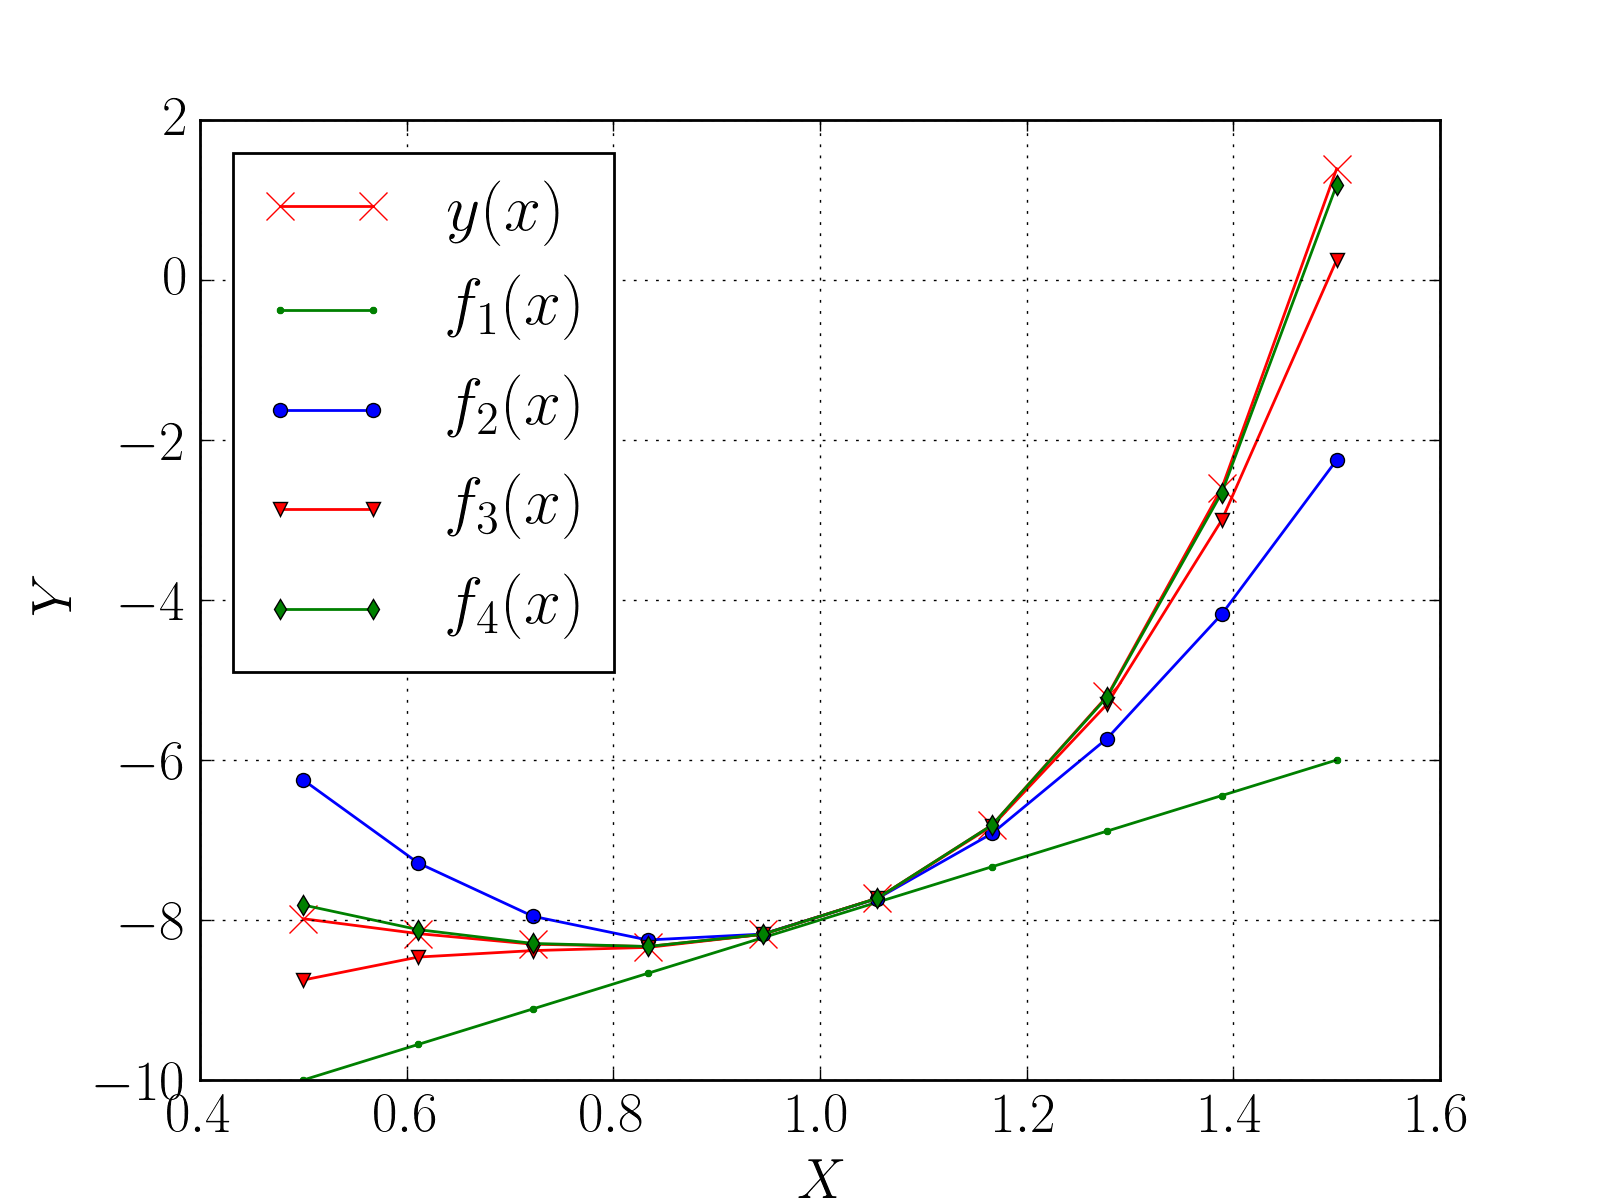
\includegraphics[width=\linewidth]{pic/taylor_1}
  \caption{График функий $y(x)$ и аппрокимирующих полиномов}
  \label{pic:taylor1}
\end{figure}

\newpage


\subsection{Получение отрезка ряда Тейлора для функции многих переменных}

Выполним подстановку выражения $z = a_1x_1 + a_2x_2$ в функцию $y = z^6 - 2z - 7$.
В результате получим:
\begin{equation}
  \label{eq:main_eq}
  z (x_1, x_2) = (a_1 x_1 + a_2 x_2)^6 - 2(a_1 x_1 + a_2 x_2) - 7.
\end{equation}

\vspace{9mm}

Для того, чтобы записать отрезок ряда Тейлора для функции (\ref{eq:main_eq}) найдём
смешенные производные этой функции до 3-го порядка включительно:
\begin{align*}
  z'_{x_1} &= 6a_1(a_1 x_1 + a_2 x_2)^5 - 2a_1,     &z'_{x_2}& = 6a_2(a_1 x_1 + a_2 x_2)^5 - 2a_2, \\
  z''_{x_1^2} &= 30a_1^2(a_1 x_1 + a_2 x_2)^4,      &z''_{x_2^2}& = 30a_2^2(a_1 x_1 + a_2 x_2)^4, \\
  z''_{x_1 x_2} &= 30 a_1 a_2 (a_1 x_1 + a_2 x_2)^4, \\
  z'''_{x_1^3} &= 120 a_1^3 (a_1 x_1 + a_2 x_2)^3,  &z'''_{x_2^3}& = 120 a_2^3 (a_1 x_1 + a_2 x_2)^3, \\
  z'''_{x_1^2 x_2} &= 120 a_1^2 a_2 (a_1 x_1 + a_2 x_2)^3,  &z'''_{x_1 x_2^2}& = 120 a_1 a_2^2 (a_1 x_1 + a_2 x_2)^3.
\end{align*}

\vspace{9mm}

Искомый отрезок ряда Тейлора для функции (\ref{eq:main_eq}) запишется так:
\begin{align*}
  &z(x_1, x_2) \sim z(a_1, a_2) + z'_{x_1}(a_1, a_2)(x-a_1) + z'_{x_2}(a_1, a_2)(x-a_2) + \\
  +& \dfrac{1}{2} \Big[ z''_{x_1}(a_1, a_2) (x-a_1)^2 + 2 \cdot z''_{x_1 x_2}(a_1, a_2) (x-a_1)(x-a_2) + z''_{x_2}(a_1, a_2) (x-a_2)^2 \Big] + \\
  +& \dfrac{1}{2 \cdot 3} \Big[  z'''_{x_1}(a_1, a_2)(x-a_1)^3 + z'''_{x_2}(a_1, a_2)(x-a_2)^3 + \\
  +& 3 \cdot z'''_{x_1^2 x_2}(a_1, a_2) (x-a_1)^2(x-a_2) + 3 \cdot z'''_{x_1 x_2^2}(a_1, a_2) (x-a_1)(x-a_2)^2 \Big]. \\ 
\end{align*}

\newpage


\subsection{Аппроксимация функции $z (x_1, x_2)$ отрезками ряда Тейлора.
  Построение графиков}

На рисунке~\ref{pic:real2} приведен график функции $z (x_1, x_2)$.
На рисунках~\ref{pic:taylor20}--\ref{pic:taylor23} изображены графики
отрезков ряда Тейлора для функции $z (x_1, x_2)$ с различным количеством
входящих членов.

\begin{figure}[h!]
  \centering
  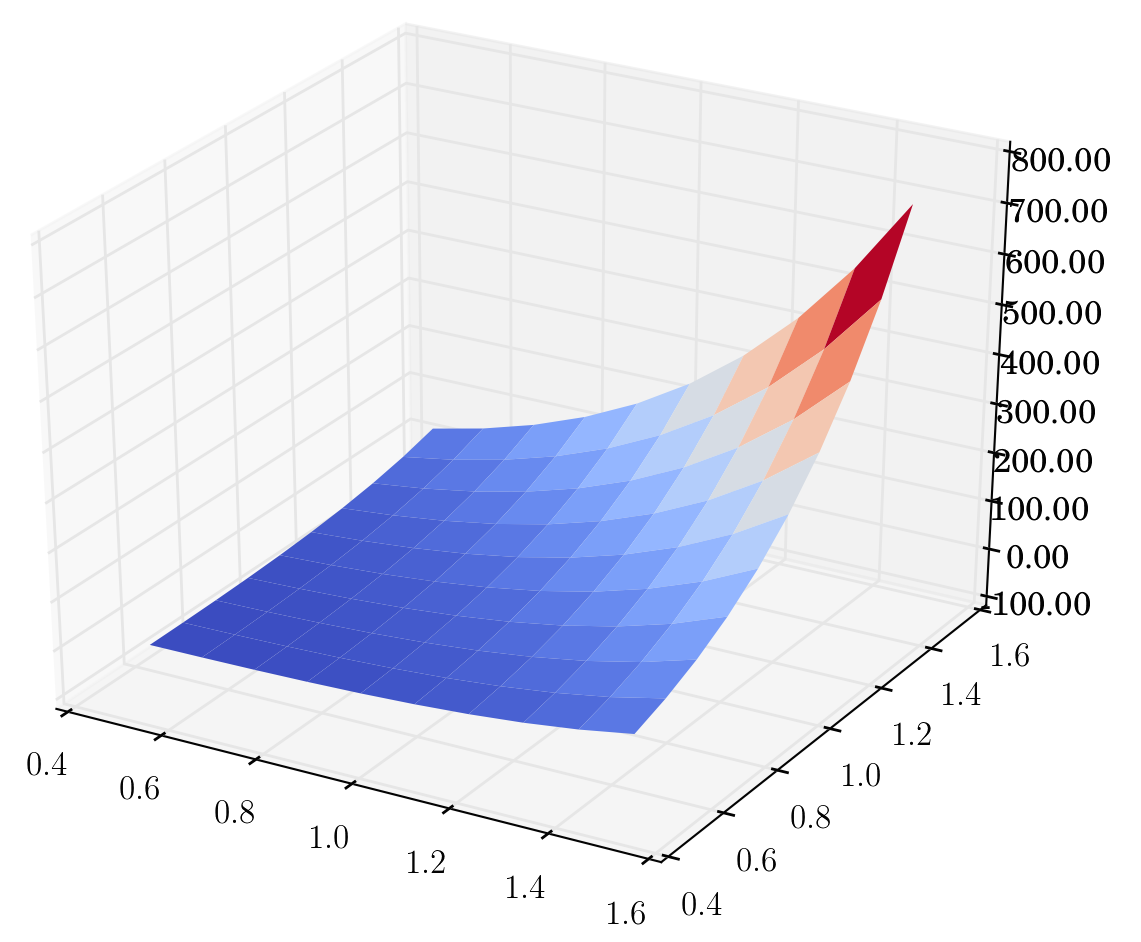
\includegraphics[width=0.55\linewidth]{pic/real_2}
  \caption{График функций $z(x_1, x_2)$}
  \label{pic:real2}
\end{figure}

\begin{figure}[h!]
  \centering
  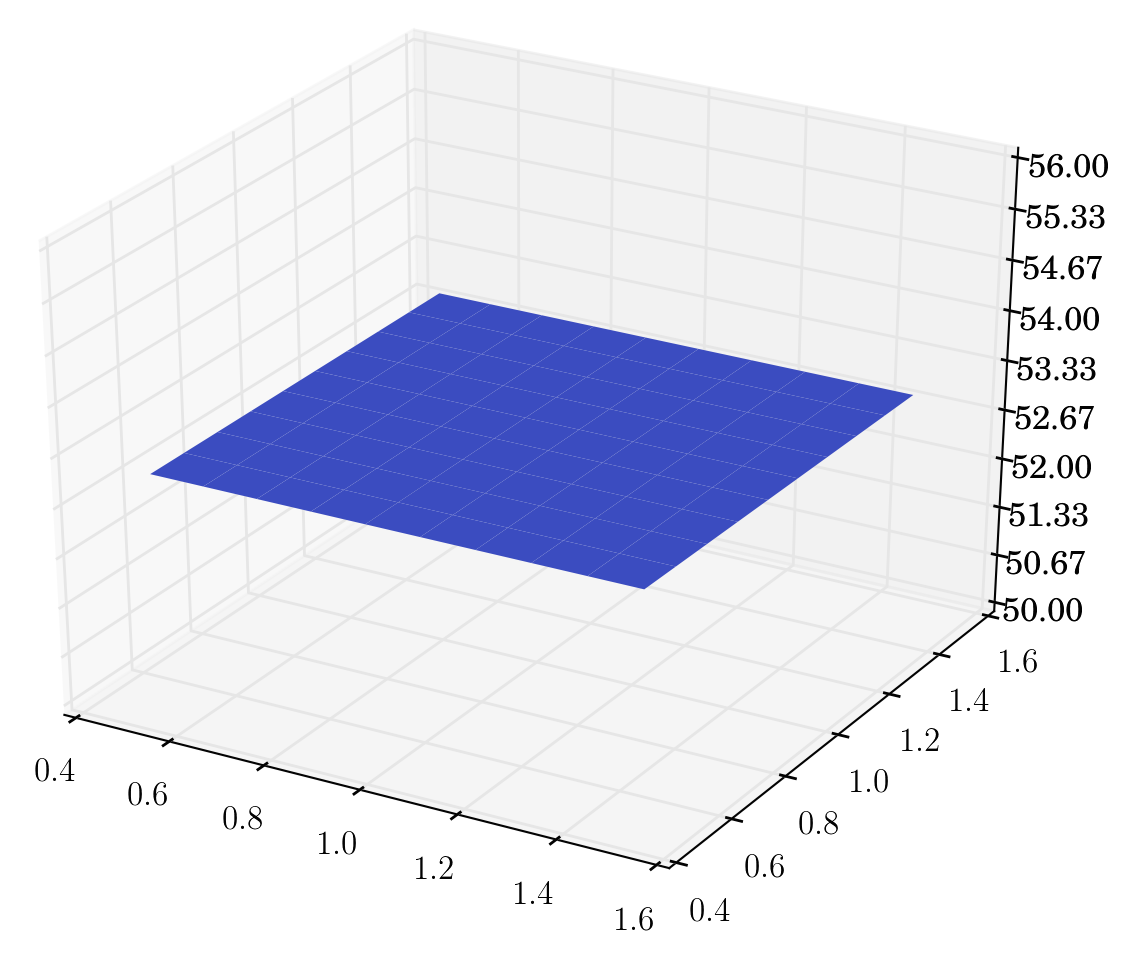
\includegraphics[width=0.55\linewidth]{pic/taylor_2_0}
  \caption{График отрезка ряда Тейлора нулевой степени \\ для функции $z(x_1, x_2)$}
  \label{pic:taylor20}
\end{figure}

\newpage

\begin{figure}[h!]
  \centering
  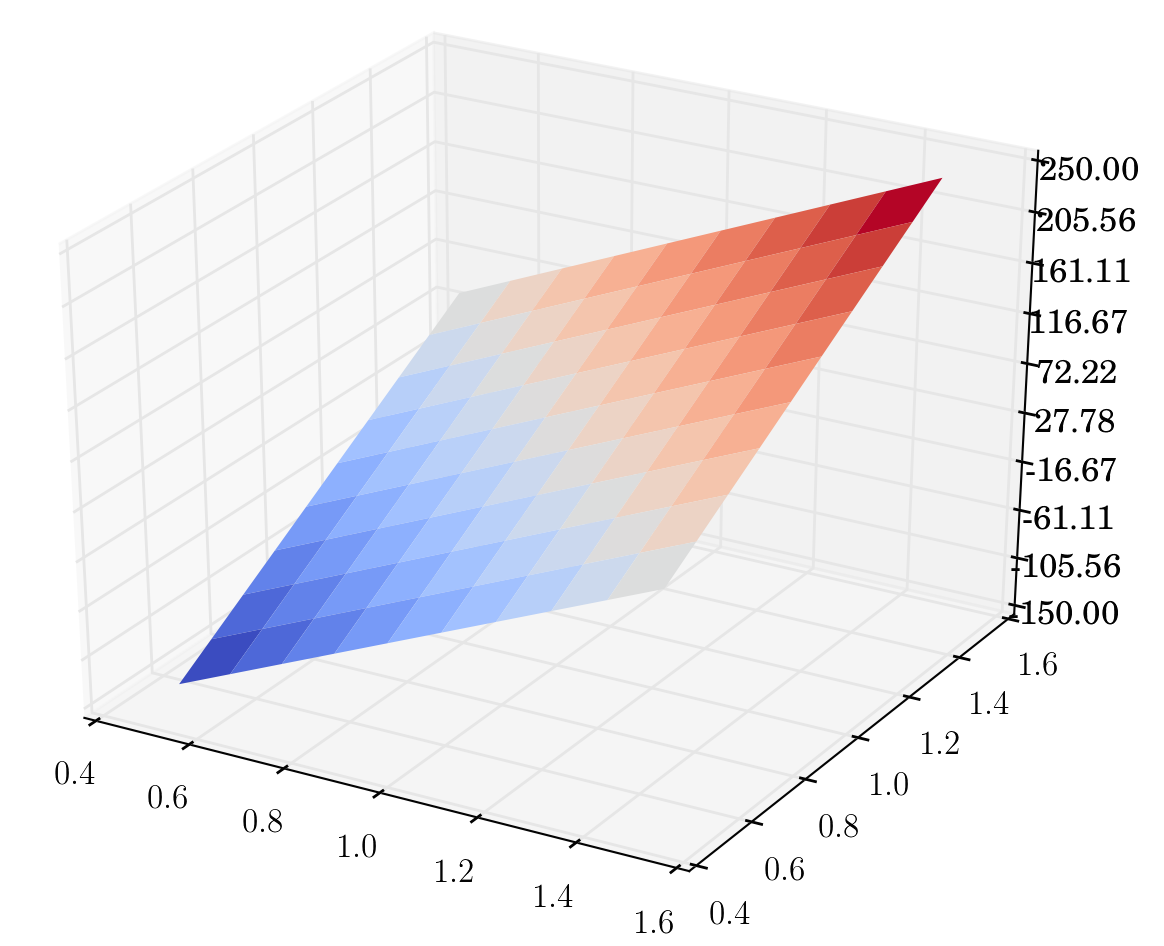
\includegraphics[width=0.71\linewidth]{pic/taylor_2_1}
  \caption{График отрезка ряда Тейлора для функции $z(x_1, x_2)$ \\ до первой степени включительно}
\end{figure}

\begin{figure}[h!]
  \centering
  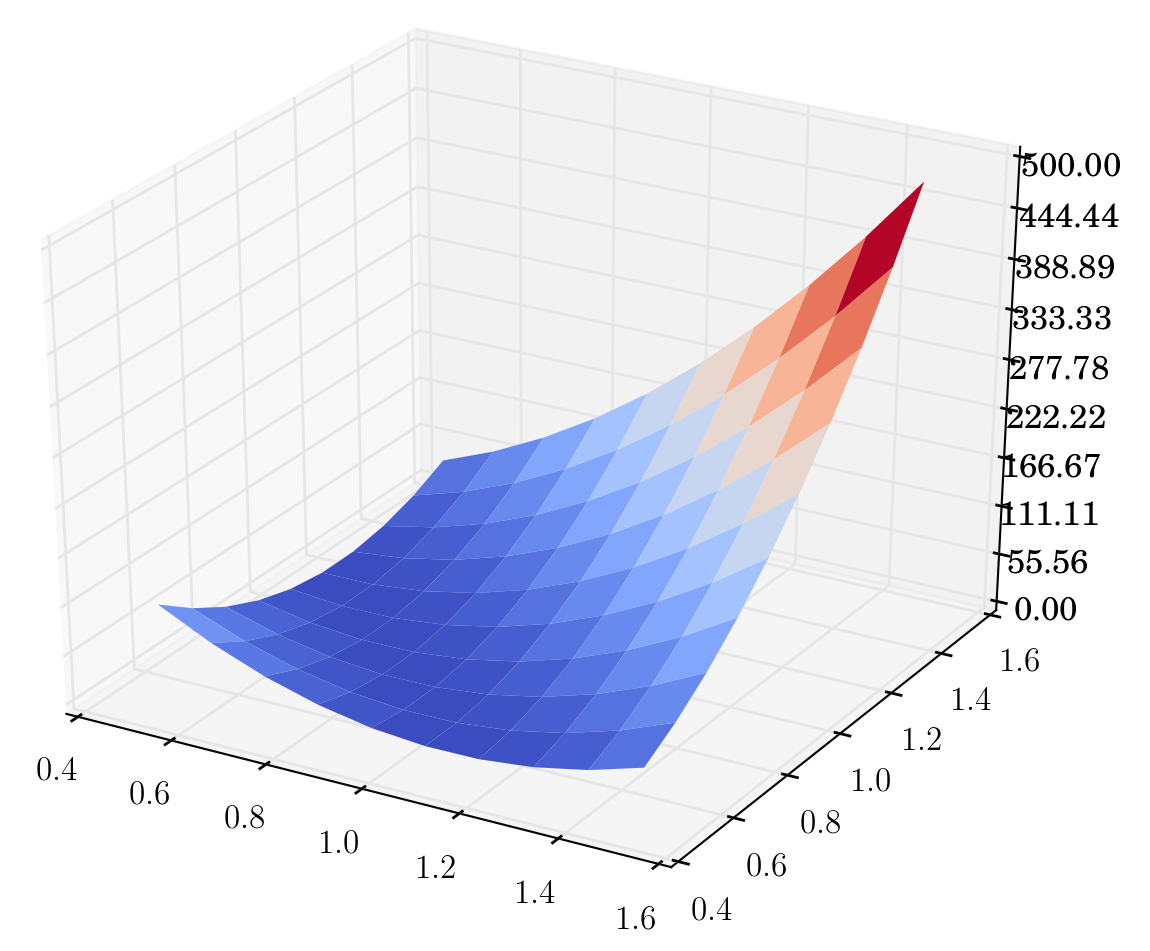
\includegraphics[width=0.71\linewidth]{pic/taylor_2_2}
  \caption{График отрезка ряда Тейлора для функции $z(x_1, x_2)$ \\ до второй степени включительно}
\end{figure}

\newpage

\begin{figure}[h!]
  \centering
  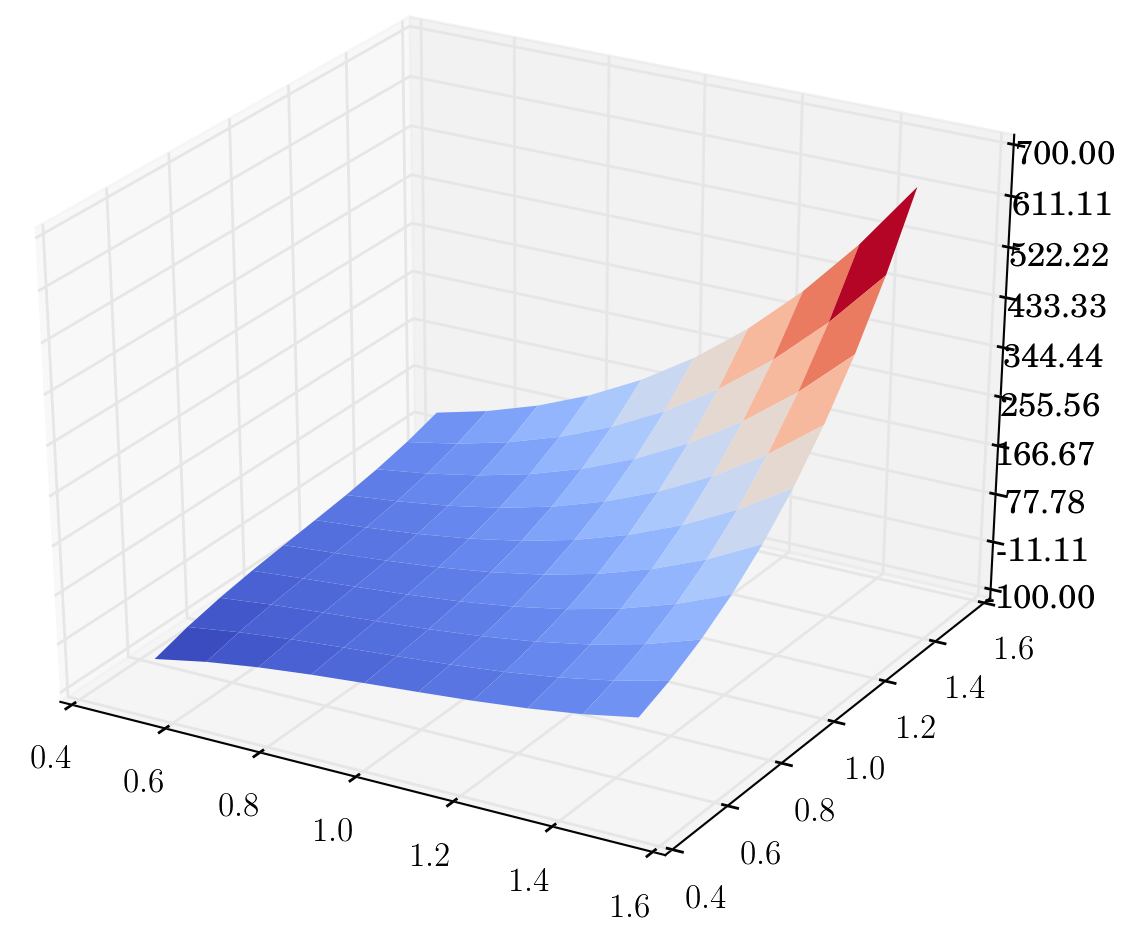
\includegraphics[width=1\linewidth]{pic/taylor_2_3}
  \caption{График отрезка ряда Тейлора для функции $z(x_1, x_2)$ \\ до третьей степени включительно}
  \label{pic:taylor23}
\end{figure}

Исходный код разработанной программы приведен в приложениях А~и~Б.
